\documentclass[aspectratio=169]{beamer}

\usetheme{Singapore} 
\usecolortheme{orchid} % seagull
\usepackage{csquotes, graphicx, booktabs, epstopdf} 
\usepackage{amsmath,amssymb,amsthm}
%% Font
\usefonttheme{professionalfonts} 
\usepackage{xeCJK} 
\setCJKmainfont{KaiTi}
\usepackage{fouriernc}
\setsansfont{Calibri}

%%% defines highlight command to set text blue
\definecolor{MyRed}{rgb}{0.4,0,0.1} 
\definecolor{MyBlue}{rgb}{0,0.2,0.6}
\newcommand{\highlight}[1]{{\color{red}{#1}}} 
	%Instructions: \alert{}, \highlight{}
	
%%%%%%% commands defining backup slides so that frame numbering is correct
\newcommand{\backupbegin}{
	\newcounter{framenumberappendix}
	\setcounter{framenumberappendix}{\value{framenumber}}
}
\newcommand{\backupend}{
	\addtocounter{framenumberappendix}{-\value{framenumber}}
	\addtocounter{framenumber}{\value{framenumberappendix}}
}
%%%% end of defining backup slides

%Specify figure caption
\setbeamertemplate{caption}{\insertcaption} %remove caption's label "Figure".
\setbeamerfont{caption}{size=\scriptsize,shape=\itshape,series=\bfseries} %sets figure caption bold and italic and makes it smaller
\setbeamertemplate{sidebar right}{}
\setbeamertemplate{footline}{%
\hfill\usebeamertemplate***{navigation symbols}
\hspace{1cm}\insertframenumber{}/\inserttotalframenumber}

% --------------------
% Overall information
% --------------------
\title{The Endogenous Grid Method for Discrete-Continuous Dynamic Choice Models with (or without) Taste Shocks, Quantitative Economics, 2017}
\author{Summarized by Wenzhi Wang} 
\institute{M.Phil. Student at the University of Oxford}
\date{May 5, 2023}

\begin{document}
	
\begin{frame}
	\titlepage
\end{frame}

\begin{frame}{Table of Contents}
	\setbeamertemplate{section in toc}[sections numbered]
	\tableofcontents %[hideallsubsections]
\end{frame}



\section[Deterministic Model]{A Deterministic Model of Consumption-Savings and Retirement}

\begin{frame}{The Sequential Problem}

	\begin{itemize}
		\item Consider the discrete-continuous (DC) dynamic optimization problem.
		\begin{equation} \label{1}
			\max _{\left\{c_t, d_t\right\}_{t=1}^T} \sum_{t=1}^T \beta^t\left(\log \left(c_t\right)-\delta d_t\right),
		\end{equation}
		involving choices of consumption $c_t$ and whether to keep working $d_t$. Let $d_t=0$ denote retirement, let $d_t = 1$ denote continued work, and let $\delta >0$ be the disutility of work. We assume retirement is absorbing.
		\item A sequence of period-specific borrowing constraints, $c_t \leq M_t$, where $$M_t = R(M_{t-1} - c_{t-1}) + yd_{t-1}$$ is consumer's consumable resources (wealth) at the beginning of period $t$. 
		\item The continuous consumption decision and discrete retirement decision are made at the start of each period, whereas interest earnings and labor income are paid at the end of the period.
	\end{itemize}

\end{frame}

\begin{frame}{The Functional Problem}

	\begin{itemize}
		\item Let $V_t(M)$ and $W_t(M)$ be the expected discounted lifetime utility of a worker and a retiree, respectively, in period t of their life.
		\item The Bellman equation for $V_t(M)$ is 
		\begin{equation}\small
			\label{2}
			V_t(M)=\max \left\{v_t(M, 0), v_t(M, 1)\right\},
		\end{equation}
		where the \highlight{choice-specific value functions}  $v_t(M, d), d \in \left\{ 0, 1\right\}$ are given by 
		\begin{equation}\small
			\label{3}
			 v_t(M, 0)=\max _{0 \leq c \leq M}\left\{\log (c)+\beta W_{t+1}(R(M-c))\right\},
		\end{equation}
		\begin{equation}\small
			\label{4}
			v_t(M, 1)=\max _{0 \leq c \leq M}\left\{\log (c)-\delta+\beta V_{t+1}(R(M-c)+y)\right\} .
		\end{equation}
		\item The Bellman equation for $W_t(M)$ is 
		\begin{equation}\small
			\label{5}
			\max _{0 \leq c \leq M}\left\{\log (c)+\beta W_{t+1}(R(M-c))\right\}.
		\end{equation}
		\item RHS of Equation \ref{3} is identical of that of Equation \ref{5}. Therefore, we have $W_t(M) = v_t(M, 0)$, and the consumption function of the retiree is identical to the choice-specific consumption function of the worker who decided to retire, $c_t(M, 0)$.
	\end{itemize}

\end{frame}

\begin{frame}{Kinks and Discontinuities}
	
\begin{itemize}
	\item Even if $v_t(M, 0)$ and $v_t(M, 1)$ are concave functions of $M$, the value function as the maximum of these two concave functions will generally not be globally concave.
	\item Further, $V_t(M)$ will generally have a kink point at the value $M = \overline{M}_t$ where the two choice-specific value functions cross, that is, $v_t(\overline{M}_t, 1) = v_t(\overline{M}_t, 0)$. We refer to these as \highlight{primary kinks}  because they constitute optimal retirement thresholds for the worker in each period $t$. 
	\item The worker is indifferent between retiring and working at the primary kink $\overline{M}_t$, and $V_t(M)$ is nondifferentiable at this point. However, the left and right hand side derivatives, $V_t^{-}(M)$ and $V_t^{+}(M)$, exist and satisfy $V_t^{-}(M) < V_t^{+}(M)$.
	\item The discontinuity in the derivative of $V_t(M)$ at $\overline{M}_t$ leads to a discontinuity in the optimal consumption function in the previous period $t - 1$ because the Bellman equation for $V_{t-1}(M)$ depends on $V_t(M)$. In turn, this causes a kink in $V_{t-1}(M)$ that we label a \highlight{secondary kink} since it is a reflection of the primary kink in $V_t(M)$.
\end{itemize}
	
\end{frame}

\begin{frame}{Analytical Solution to the Retirement Problem}\footnotesize
	
	\begin{theorem} \label{thm1}
		Theorem 1. Assume that income and disutility of work are time-invariant, the discount factor $\beta$ and the disutility of work $\delta$ are not too large, that is, 
		\begin{equation}
			\label{6}
			\beta R \leq 1 \quad \text { and } \quad \delta<(1+\beta) \log (1+\beta),
		\end{equation}
		and instantaneous utility is given by $u(c) = log(c)$. Then for $\tau \in \{1, \ldots, T\}$ the optimal consumption rule in the worker's problem \ref{2}-\ref{4} is given by 
			
	\end{theorem}
\end{frame}

\begin{frame}{Analytical Solution to the Retirement Problem}\footnotesize
	
	\begin{theorem}
				
		\begin{equation}
			\label{7}
			\begin{aligned}
				c_{T- \tau}^w(M) = 
				\begin{cases}
					M & \text { if } M \leq y / R \beta, \\
					{[M+y / R] /(1+\beta)} & \text { if } y / R \beta \leq M \leq\overline{M}_{T-\tau}^{l_1}, \\
					{\left[M+y\left(1 / R+1 / R^2\right)\right] /\left(1+\beta+\beta^2\right)} &\text { if } \overline{M}_{T-\tau}^{l_1} \leq M \leq \overline{M}_{T-\tau}^{l_2}, \\
					\cdots & \cdots \\
					{\left[M+y\left(\sum_{i=1}^{\tau-1}R^{-i}\right)\right]\left(\sum_{i=0}^{\tau-1} \beta^i\right)^{-1}} & \text { if } \overline{M}_{T-\tau}^{l_{\tau-2}} \leq M \leq \overline{M}_{T-\tau}^{l_{\tau-1}}, \\
					{\left[M+y\left(\sum_{i=1}^\tau R^{-i}\right)\right]\left(\sum_{i=0}^\tau \beta^i\right)^{-1}} & \text { if } \overline{M}_{T-\tau}^{l_{\tau-1}} \leq M<\overline{M}_{T-\tau}^{r_{\tau-1}}, \\
					{\left[M+y\left(\sum_{i=1}^{\tau-1} R^{-i}\right)\right]\left(\sum_{i=0}^\tau \beta^i\right)^{-1}} & \text { if } \overline{M}_{T-\tau}^{r_{\tau-1}} \leq M<\overline{M}_{T-\tau}^{r_{\tau-2}}, \\
					\cdots & \cdots \\
					{\left[M+y\left(1 / R+1 / R^2\right)\right]\left(\sum_{i=0}^\tau\beta^i\right)^{-1}} & \text { if } \overline{M}_{T-\tau}^{r_2} \leq M<\overline{M}_{T-\tau}^{r_1}, \\
					{[M+y / R]\left(\sum_{i=0}^\tau \beta^i\right)^{-1}} & \text { if }\overline{M}_{T-\tau}^{r_1} \leq M<\overline{M}_{T-\tau}, \\
					{M\left(\sum_{i=0}^\tau \beta^i\right)^{-1}} & \text { if } M \geq\overline{M}_{T-\tau} .
				\end{cases}
			\end{aligned}
		\end{equation}
		
	\end{theorem}
\end{frame}

\begin{frame}{Analytical Solution to the Retirement Problem}\footnotesize
	\begin{theorem}
		
		The segment boundaries are totally ordered with 
		\begin{equation}\label{8}
			\frac{y}{R\beta}<\overline{M}_{T-\tau}^{l_1}<\cdots<\overline{M}_{T-\tau}^{l_{\tau-\tau}}<\overline{M}_{T-\tau}^{r_{T-1}}<\cdots<\overline{M}_{T-\tau}^{r_1}<\overline{M}_{T-\tau},
		\end{equation}
		and the rightmost threshold $\overline{M}_{T-\tau}$, given by
		\begin{equation}
			\overline{M}_{T-\tau}=\frac{(y / R) e^{-K}}{1-e^{-K}}, \quad \text { where } K=\delta\left(\sum_{i=0}^\tau \beta^i\right)^{-1},
		\end{equation}
		defines the smallest level of wealth sufficient to induce the consumer to retire at age $t = T - \tau$.

	\end{theorem}
\end{frame}

\begin{frame}{Analytical Optimal Consumption Function}

	\begin{itemize}
		\item Theorem 1 establishes that the optimal consumption rule of the worker $c_{T-\tau}(M, 1)$ is piecewise linear in $M$, and in period $t$ consists of $2(T-t)+1$ segments. 
		\item The first segment where $M<\frac{y}{R\beta}$ is the credit constrained region where the agent consumes all available wealth and does not save.
		\item The next $T-t-1$ segments are demarcated by the \highlight{liquidity constraint kink points} $\overline{M}_t^{l_j}$ that define values of $M$ at which the consumer is liquidity constrained at age $t+j$ but not at any earlier age. 
		\item The remaining segments are defined by the secondary kinks, $\overline{M}_t^{r_j}, j=1, \ldots, T-t-1$, and represent the largest level of saving for which it is optimal to retire at age $t+j$ but not at any earlier age.
		\item Finally, $\overline{M}_t$ is the retirement threshold, which denotes the minimum level of wealth that is required to retire.
		\item The optimal consumption function is discontinuous at points $\overline{M}_t^{r_j}$ and $\overline{M}_t$, so in total there are $T - t$ downward jumps in the consumption function.

	\end{itemize}
	
\end{frame}

\begin{frame}{Analytical Value Function $V_t(M)$}

	\begin{itemize}
		\item Theorem \ref{thm1} implies that the value function $V_t(M)$ is piecewise logarithmic with the same kink points, and can be written as $V_t(M) = B_t \log(c_t (M, d)) + C_t$ for constants $(B_t, C_t)$ that depend on the region that $M$ falls into.
		\item The function $V_t(M)$ has one primary kink at the optimal retirement threshold $\overline{M}_t$ and $T-t-1$ secondary kinks at $\overline{M}_t^{r_j}, j = 1, \ldots, T-t-1$.
		\item In addition, there are $T-t$ kinks related to current and future liquidity constraints at $M=\frac{y}{R\beta}$ and $\overline{M}_t^{l_j}, j = 1, \ldots, T-t-1$.

	\end{itemize}
	
\end{frame}

\section[DC-EGM without Taste Shocks]{DC-EGM Algorithm for the Deterministic Model}

\begin{frame}{Euler Equations}

	\begin{itemize}
		\item DC-EGM is a backward induction algorithm that uses the \highlight{inverted Euler equation} to sequentially compute the choice-specific value functions $v_t(M, d)$ and the corresponding choice-specific consumption functions $c_t(M, d)$ starting at the last period of life, $T$.
		\item A worker who remains working satisfies the Euler equation is 
		\begin{equation}
			\label{10}
			\begin{aligned}
				0 & =u^{\prime}(c)-\beta R u^{\prime}\left(c_{t+1}^w(R(M-c)+y)\right) \\
				& =\frac{1}{c}-\frac{\beta R}{c_{t+1}^w(R(M-c)+y)} .
			\end{aligned}
		\end{equation}
		\item For a worker who decides to retire, the Euler equation is 
		\begin{equation}
			\label{11}
			\begin{aligned}
				0 & =u^{\prime}(c)-\beta R u^{\prime}\left(c_{t+1}^r(R(M-c))\right) \\
				& =\frac{1}{c}-\frac{\beta R}{c_{t+1}^r(R(M-c))} .
				\end{aligned}
		\end{equation}
		
	\end{itemize}
	
\end{frame}

\begin{frame}{The Endogenous Grid Method: General Idea}
	\begin{itemize}
		\item Given the period $t+1$ optimal consumption functions, i.e., $c_{t+1}^w(M)$ for workers and $c_{t+1}^r(M)$ for retirees, the solutions to these Euler equations \ref{10} and \ref{11} yield the period $t$ choice-specific consumption functions of the worker, $c_t(M, d).$ 
		\item When an inverse of the marginal utility is closed-form, specifying an exogenous grid over end-of-period saving $A = M-c$ facilitates solving for optimal current consumption in closed form without resorting to iterative numerical methods. 
	\end{itemize}
\end{frame}

\begin{frame}{Solution in Period $T$}
	\begin{itemize}
		\item Consider the terminal period $T$. The optimal consumption rule is to consume all available wealth and, thus, is given by $c_T (M, d) = M$. With positive disutility of working, all agents retire since income is paid at the end of the period. This $T$ period solution is the base for backward induction.
			\end{itemize}
\end{frame}

\begin{frame}{Retirees: from Period $T$ to $T-1$} \small
	
	Consider a retiree in time $T-1$. 

	\begin{itemize}
		
		\item In EGM, we first construct an exogenous grid over savings $A= M-c$. Let $\overrightarrow{A} = \{ A_1, \ldots, A_J \}$ denote the exogenous grid over savings. Euler equation \ref{11} can be solved for $c$, $\overline{c}_{T-1}^r (A_{j})$ for each point $A_j$. (The solution is easily seen to be $\overline{c}_{T-1}^r (A_{j})= \frac{A_j}{\beta}$.)
		\item Next, we need to get $M_{j, T-1} \in \overrightarrow{M}_{T-1}$, where $\overrightarrow{M}_{T-1}$ is the endogenous grid implied by the exogenous grid over savings $\overrightarrow{A}$. To be specific, we have $$M_{j, T-1} = A_j + \overline{c}_{T-1}^r(A_{j}), $$ now we can map $A_j$ to $M_{j, T-1}$, and therefore transform the function $\overline{c}_{T-1}^r(A_{j})$ to $c_{T-1}^r(M_{j, T-1})$ .
		\item Moreover, at the points of the endogenous grid $\overrightarrow{M}_{t}$, and with linear interpolation, EGM produces an exact solution $c_{T-1}^r(M) = \frac{M}{1+\beta}$. .
	\end{itemize}
	
\end{frame}

\begin{frame}{Workers: from Period $T$ to $T-1$}

	Now consider a worker in period $T-1$. 

	\begin{itemize}\small
		
		\item Apply ``standard EGM'' to solve the optimal consumption rule of a worker $c_{T-1}(M,d)$ for each of the discrete decisions $d$, using Euler equation (\ref{10}) or (\ref{11}). 
		\item Similar to the retiree case, with linear interpolation, this also results in exact solutions.

	\end{itemize}

	To ensure that the credit constraint $c_{T-1} \leq M$ is satisfied, we need the following steps. 
	\begin{itemize}\small
		\item First, from (\ref{10}) it follows that invoking the EGM algorithm with zero savings, $A_j=0$, produces an endogenous point $M_{j, T-1} = \frac{y}{R\beta}$. 
		\item Next, as we show in Theorem \ref{thm2}, savings as a function of wealth must be nondecreasing, and, therefore, for $M\leq \frac{y}{R\beta}$, the savings must remain zero, that is, $c_{T-1}(M) = M$.
		\item Therefore, it is sufficient to add a point $M_{0, T-1} = 0$ to the endogenous grid $\overrightarrow{M}_{T-1}$, and set the corresponding optimal consumption $c_{T-1}(M_{0, T-1}, 1) = M_{0, T-1}=0$. (\highlight{Linear Interpolation Matters!})
	\end{itemize}
\end{frame}

\begin{frame}{Difference in DC-EGM from Standard EGM}\small
	\begin{itemize}
		\item Now we have obtained the decision-specific consumption functions $c_t(M_{j,t}^d, d)$ defined over decision-specific endogenous grids $\overrightarrow{M}_t^d = \{M_{1,t}^d, \ldots, M_{J,t}^d\}$.
		\item What is different about DC-EGM is that we need to compare the choice-specific value functions $v_t(M,0)$ and $v_t(M, 1)$ so as to locate the threshold level of wealth when it becomes optimal to retire, $\overline{M}_t$.

	\end{itemize}
\end{frame}

\begin{frame}{Difference in DC-EGM from Standard EGM}\small
	\begin{itemize}
		\item DC-EGM constructs approximations to $v_t(M,0)$ and $v_t(M, 1)$ over the respective endogenous grids $\overrightarrow{M}_t^0$ and $\overrightarrow{M}_t^1$ alongside the calculation of the optimal consumption functions $c_t(M, 0)$ and $c_t(M, 1)$ by substituting the latter into the Bellman equations (\ref{3}) and (\ref{4}). 
		\item Then, using the decision-specific value functions, we then find the optimal retirement threshold $\overline{M}_t$ by finding the point of intersection of the two decision-specific value functions, $v_t(M,0) = v_t(M, 1)$.
		\item The overall value function for the worker $V_t(M)$ is then computed as an \highlight{upper envelope} of the two choice-specific value functions $v_t(M, d)$, each defined over the endogenous grid $\overrightarrow{M}_t^d$.
		\item Similarly, the \highlight{optimal consumption function} of the worker $c_{T-1}^w(M)$ is combined from choice-specific consumption functions $c_{T-1}(M,1)$ and $c_{T-1}(M,0)$ depending on whether the level of wealth $M$ is below or above the primary kink point $\overline{M}_{T-1}$, fully in line with formula \ref{7} of Theorem \ref{thm1} for $\tau=1$.
	\end{itemize}
\end{frame}



\begin{frame}{Difficulties in Period $T-2$}
	\begin{itemize}
		\item Complication: the \highlight{emergence of secondary kinks} due to \highlight{multiple local optima} for $c$ in the Bellman equation \ref{4}.
		\item Recall that $V_t(M)$ is the maximum of decision-specific value functions and is not globally concave. In particular, $V_{T-1}(M)$ has a nonconcave region near $\overline{M}_{T-1}$, where the decision-specific value functions $v_{T-1}(M,0)$ and $v_{T-1}(M,1)$ cross.
		\item This implies that at time $T-2$ when we search over $c$ to maximize $\log(c) + \beta V_{T-1}(R(M-c)+y)$ in equation \ref{4}, for some level of $M$ there will be multiple local optima for $c$ with corresponding multiple solutions to the Euler equations.
		\item Thus, DC-EGM must also take care to select the correct solution to the Euler equation corresponding to the globally optimal consumption value.
		\item \highlight{This is achieved by the calculation of the upper envelope over the overlapping segments of the decision-specific value functions that are produced from different solutions. The dominated grid points are then eliminated from the endogenous grid in a way below.}
		
	\end{itemize}
\end{frame}


\begin{frame}{Select the Right Solution to the Euler Equations} \small
	\begin{theorem} \label{thm2}
		Theorem 2 (Monotonicity of the Saving Function). Let $A_t(M, d) = M - c_t(M, d)$ denote the savings function implied by the optimal consumption function $c_t(M, d)$. If $u(c)$ is a concave function, then for each $t \in \{1, \ldots, T\}$ and each discrete choice $d \in \{0,1\}$ the optimal saving function $A_t(M, d) = M - c_t(M, d)$ is monotone nondecreasing in $M$.
	\end{theorem}
	\begin{itemize}
		\item Key second step of DC-EGM: refinement of the endogenous grid to discard the suboptimal points produced by the EGM step.
		\item Construct the upper envelope over the segments of the discrete choice-specific value function correspondence in the region of $M$ where multiple solutions were detected. The detection itself relied on checking for monotonicity of the endogenous grid.
		\item With the refined monotonic endogenous grid $\overline{M}_{T-2}^{*1}$ constructed from the upper envelope of the interpolated value functions, we obtain a close approximation to the correct optimal consumption rule $c_{T-1}^w(M)$.
		\item See Figure 1 in the original paper for more details.
	\end{itemize}
\end{frame}

\begin{frame}{Graphical Illustration of the Selection Process}
	\label{fig:upperenvelope}
	\begin{figure}[htbp!]
		\begin{minipage}{0.55\linewidth}
			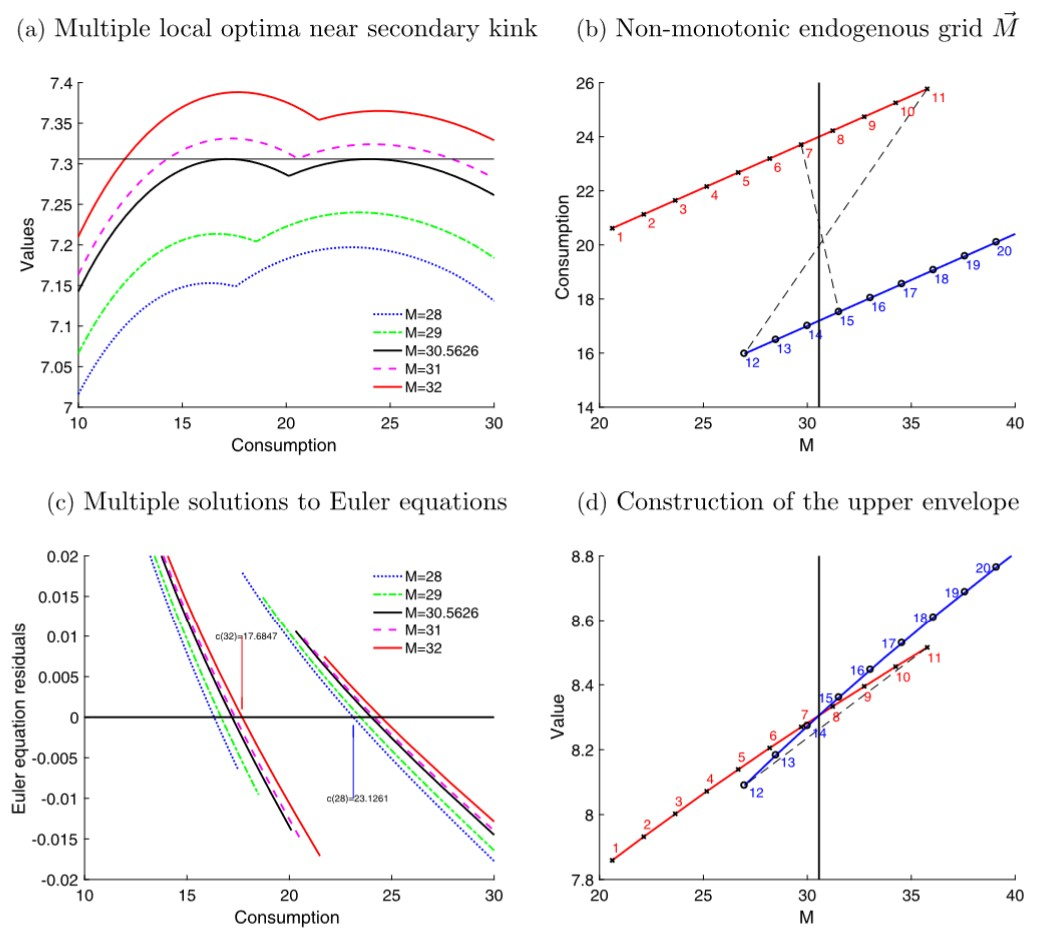
\includegraphics[scale=0.5]{fig1.jpg}
		\end{minipage}
		\begin{minipage}{0.4\linewidth}
			\begin{itemize} \small
				\item The most important step is in panel (b) and (d).
				\item We need to check monotonicity of the endogenous wealth grid for each choice and construct the upper envelope for choice-specific value function in certain regions.
				\item Link to algorithm \hyperlink{algo:upperenvelope}{\beamerreturnbutton{Upper Envelope}}. 
			\end{itemize}
		\end{minipage}
	\end{figure}
\end{frame}

\begin{frame}{Graphical Illustration of the Nonmonotonicity and Selection Process}
	\begin{figure}[htbp!]
		\begin{minipage}{0.55\linewidth}
			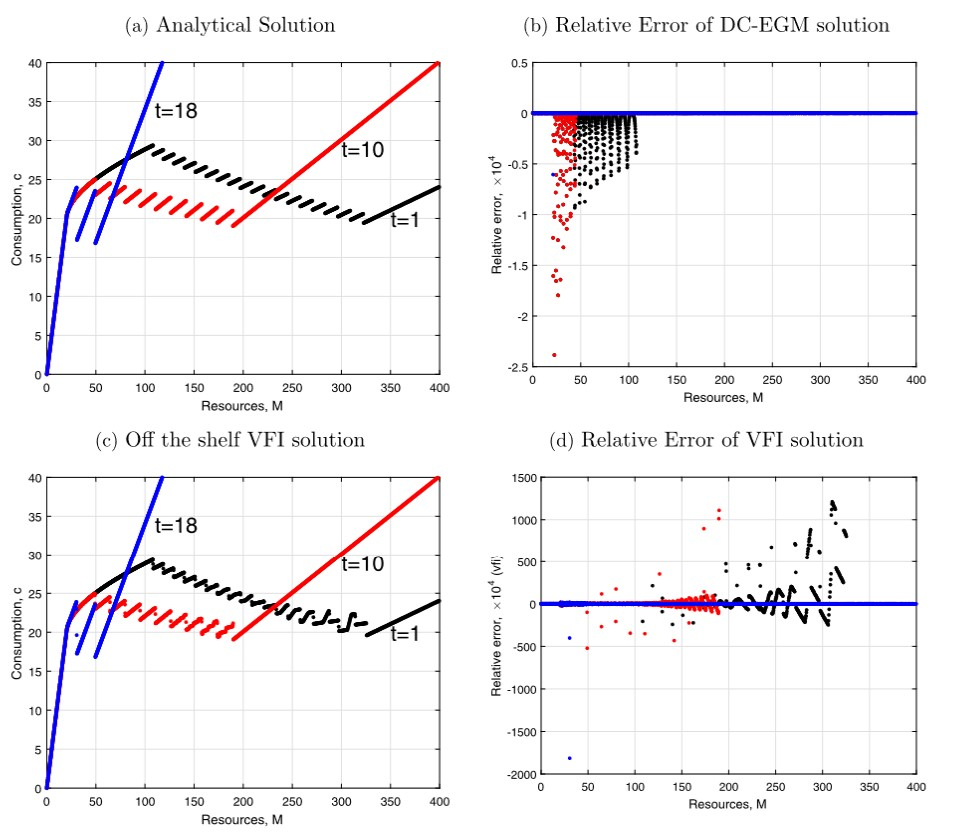
\includegraphics[scale=0.55]{fig2.jpg}
		\end{minipage}
		\begin{minipage}{0.4\linewidth}
			$R = 1, \beta = 0.98$, \\ $y = 20, T = 20$. \\ \highlight{MATLAB Implementation!!!}
		\end{minipage}
	\end{figure}
\end{frame}

\section[Stochastic Model]{A Model of Consumption-Savings and Retirement with Income and Taste Shocks}

\begin{frame}{Effects of introducint income shocks and taste shocks}
	\begin{itemize}
		\item First, because the discrete choice policy is expressed in probabilistic terms, the calculation of primary kink points is no longer needed.
		\item Second, the process of accumulation of secondary kinks is perturbed: the perturbations caused by the primary kinks that remain throughout the backward induction process in the deterministic setting ``fade out'' in the presence of shocks.
		\item Third, the calculation of expectations over random income in the problem with taste shocks can be performed with standard numerical algorithms, as opposed to the setting with random income but without taste shocks.
	\end{itemize}
\end{frame}

\begin{frame}{Income and Taste Shocks}

	For the worker's problem, the Bellman equation is 
	\begin{equation}
		\label{12}
		V_t(M, \varepsilon)=\max \left\{v_t(M, 0)+\sigma_{\varepsilon} \varepsilon(0), v_t(M, 1)+\sigma_{\varepsilon} \varepsilon(1)\right\},
	\end{equation}
	where the conditional value function for retirement, $v_t(M,0)$ is still given by \ref{3}. However, the conditional value function for remaining working, $v_t(M,0)$ now becomes
	\begin{equation}
		\label{13}
		v_t(M, 1)=\max _{0 \leq c \leq M}\left\{\log (c)-\delta+\beta \int \overline{V}_{t+1}^{\sigma_{\varepsilon}}(R(M-c)+y \eta) f(d \eta)\right\}.
	\end{equation}
	The ex ante (integrated) value function $\overline{V}_{t+1}^{\sigma_{\varepsilon}}(M)$ is 
	\begin{equation}\small
		\label{14}
		\begin{aligned}
			\overline{V}_{t+1}^{\sigma_{\varepsilon}}(M, 1) & = E_{\varepsilon} \left[ V_{t+1} (M, \varepsilon) \right] \\
			& = E_{\varepsilon} \left[\max \left\{v_{t+1}(M, 0)+\sigma_{\varepsilon} \varepsilon(0), v_{t+1}(M, 1)+\sigma_{\varepsilon} \varepsilon(1)\right\}\right] \\
			& =\sigma_{\varepsilon} \log \left(\exp \left\{\frac{v_{t+1}(M, 0)}{\sigma_{\varepsilon}}  \right\}+\exp \left\{\frac{v_{t+1}(M, 1)}{\sigma_{\varepsilon}}\right\}\right) .
		\end{aligned}
	\end{equation}
	The last equality comes from the iid extreme value distribution assumption.
\end{frame}

\begin{frame}{Elimination of Primary Kinks}
	\begin{itemize}
		\item The immediate effect of introducing extreme value taste shocks is the complete elimination of the \highlight{primary} kinks, because the location of the indifference point in equation \ref{12} is now probabilistic from the point of view of the econometrician.
		\item The discrete choice policy function is now given by the logit choice probabilities $P_t(d \mid M)$ that arise due to the distributional assumption for the taste shocks:
		\begin{equation}
			\label{15}
			P_t(d \mid M)=\frac{\exp \left\{v_t(M, d) / \sigma_{\varepsilon}\right\}}{\exp \left\{v_t(M, 1) / \sigma_{\varepsilon}\right\}+\exp \left\{v_t(M, 0) / \sigma_{\varepsilon}\right\}}, \quad d \in\{0,1\} .
		\end{equation}
		
		\item It is worth noting that the problem is still not globally concave in general, so the upper envelope calculation and the elimination of the suboptimal endogenous points is still performed as before.
	\end{itemize}
\end{frame}

\begin{frame}{Further Discussion on Shocks and Smoothness}
	\begin{itemize}
		\item The income shocks in the model also smooth out the secondary kinks during backward induction. When the agent cannot perfectly anticipate having next period wealth exactly at the kink point, the secondary kinks are not replicated perfectly in the prior periods.
		\item In the absence of taste shocks, the primary kinks cannot be avoided even if all secondary kinks are eliminated by a sufficiently high degree of uncertainty in the model.
		\item The taste shocks and other structural shocks together contribute to the reduction of the number of secondary kinks and to the alleviation of the issue of their multiplication and accumulation.
		\item Theorem 3 in the paper talks about convergence property in the extreme value smoothing process.
	\end{itemize}
\end{frame}

\section[DC-EGM with Taste Shocks]{DC-EGM Algorithm for a Model with Taste Shocks}

\begin{frame}{Smmoothed Euler Equation}
	\begin{itemize}
		\item If we continue to assume that retirement is an absorbing state, the problem of the retiree remains the same, and we focus again on the worker's problem.
		\item The smoothed Euler equation with taste and income shocks derived from equations \ref{12}, \ref{3}, and \ref{13} is 
		\begin{equation} \footnotesize
			\label{17}
			\begin{aligned}
				0= & u^{\prime}(c)-\beta R \int [u^{\prime}\left(c_{t+1}(R(M-c)+y \eta, 1)\right) P_{t+1}(1 \mid R(M-c)+y \eta)+ \\
				& u^{\prime}\left(c_{t+1}(R(M-c)+y \eta, 0)\right) P_{t+1}(0 \mid R(M-c)+y \eta)] f(d \eta) \\
				= & \frac{1}{c}-\beta R \int\left[\frac{P_{t+1}(1 \mid R(M-c)+y \eta)}{c_{t+1}(R(M-c)+y \eta, 1)}+\frac{P_{t+1}(0 \mid R(M-c)+y \eta)}{c_{t+1}(R(M-c)+y \eta, 0)}\right] f(d \eta),
			\end{aligned}
		\end{equation}
		where $P_{t+1}(d \mid M)$ and conditional choice probabilities \ref{15}.
	\end{itemize}
\end{frame}

\begin{frame}{Solution in Period $T$}
	\begin{itemize}
		\item The induction starts at the terminal period $T$ with the easily derived consumption functions $$c_T(M,0) = c_T(M, 1) = M, $$ choice-specific value functions $$v_T(M, 0) = u(M) = v_T(M,1) + \delta, $$ and the probability of remaining working $$P_{T}(1 \mid M) = \frac{1}{1 + \exp (\delta / \sigma_\varepsilon)}.$$
	\end{itemize}
\end{frame}

\begin{frame}{Backward Induction from Period $T$ to Period $T-1$}
	\begin{itemize}
		\item We choose an exogenous grid over saving $\overline{A} = \{A_1, \ldots, A_J\}$ which remains fixed throughout the backward induction process here for notational simplicity. 
		\item Compute optimal consumption $\left\{ \overline{c}_{T-1} (A_1, d), \ldots, \overline{c}_{T-1}(A_J, d) \right\}$ for each point $A_j$ and for each discrete choice $d$ by calculating the inverse marginal utility of the RHS of the Euler equations \ref{17} and \ref{11} for $d=1$ and $d=0$, respectively.
		\item Construct the endogenous grid over $M$ as $\overrightarrow{M}_{T-1}^d = ({M}_{1, T-1}^d, \ldots, {M}_{J, T-1}^d)$, where $$M_{j, T-1} = \overline{c}_{T-1}(A_j, d) + A_j, j \in \{1, \ldots, J\}.$$
	\end{itemize}
\end{frame}

\begin{frame}{Potential Selection Process}
	\begin{itemize}
		\item In period $t$, for every $d$, if the resulting mapping from grid points in $\overrightarrow{A}$ to $\overrightarrow{M}_t^d$ is monotonically increasing, then there is no violation against Theorem \ref{thm2}, and the DC-EGM method automatically reverts to the standard EGM.
		\item If $\overrightarrow{M}_t^d$ is not a monotonically increasing sequence, we apply the same upper envelope procedure over $d$ to eliminate the suboptimal elements of $\overrightarrow{M}_t^d$ 
		\item Add a point where the disjoint segments of the value function intersect. This step amounts to calculating the choice-specific value functions $v(M,d)$ alongside the consumption functions, which is achieved by plugging the computed $c_t(A_1, d)$ into the maximand of the Bellman equation \ref{13} for each point $A_j$ of the exogenous grid on savings.
		\item After the choice-specific consumption and value functions $c(M, d)$ and $v(M, d)$ are computed on the monotonic endogenous grids $\overrightarrow{M}_t^{*d}$, the period $t$ iteration of the DC-EGM algorithm is complete.
	\end{itemize}
\end{frame}

\begin{frame}{Pseudo Codes for EGM Algorithm: Set up the Iteration}
	\begin{figure}
		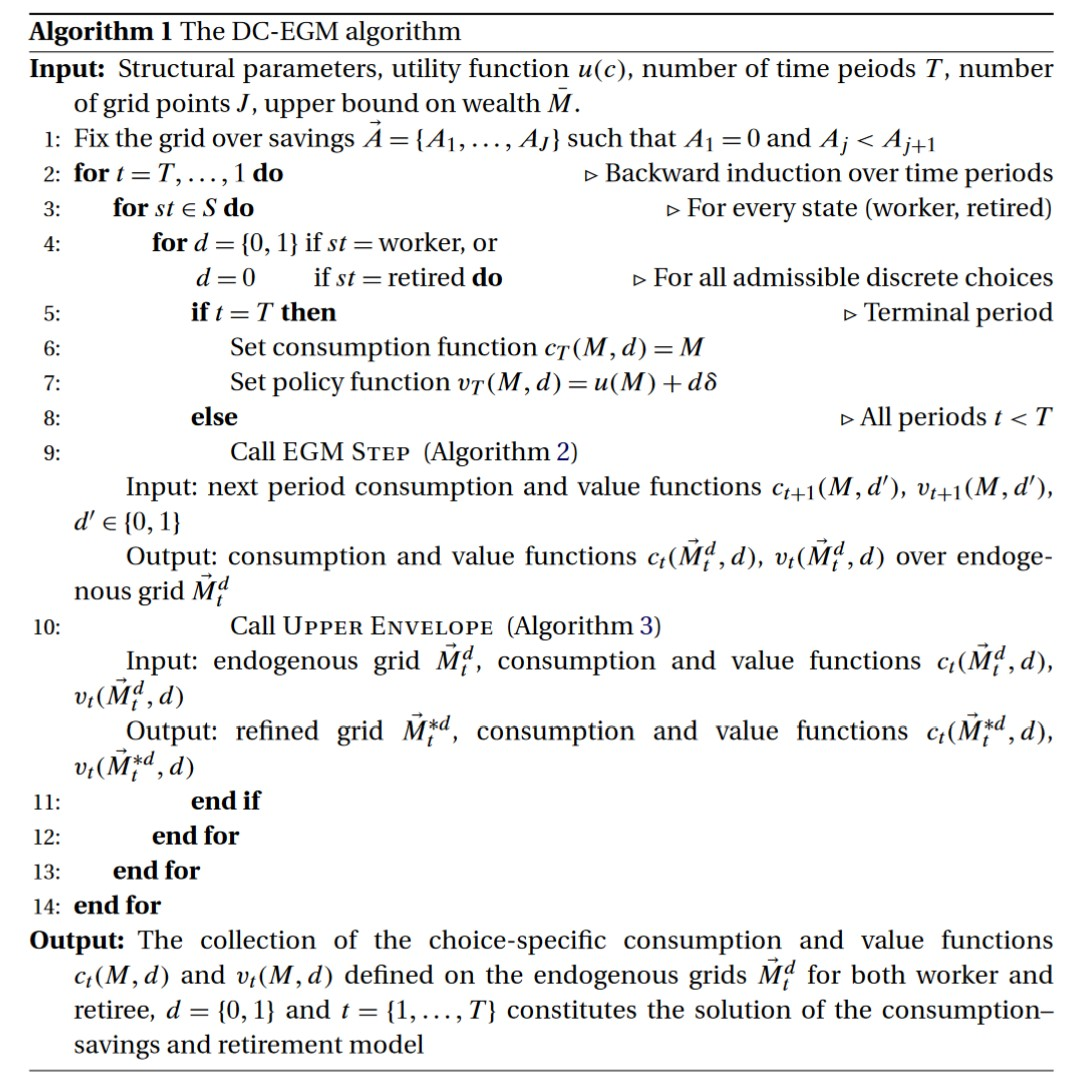
\includegraphics[scale=0.45]{algorithm1.jpg}
	\end{figure}
\end{frame}

\begin{frame}{Pseudo Codes for EGM Algorithm: EGM}
	\begin{figure}
		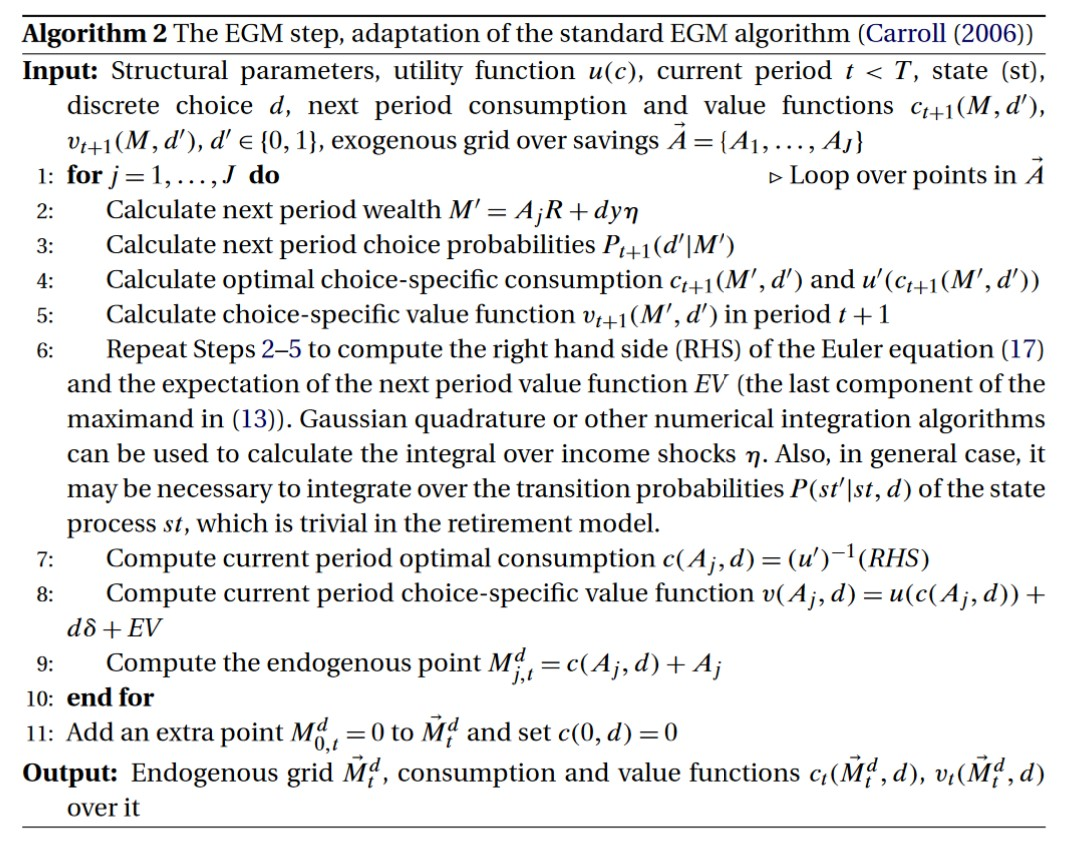
\includegraphics[scale=0.5]{algorithm2.jpg}
	\end{figure}
\end{frame}

\begin{frame}{Pseudo Codes for EGM Algorithm: Upper Envelope}
	\label{algo:upperenvelope}
	\begin{figure}
		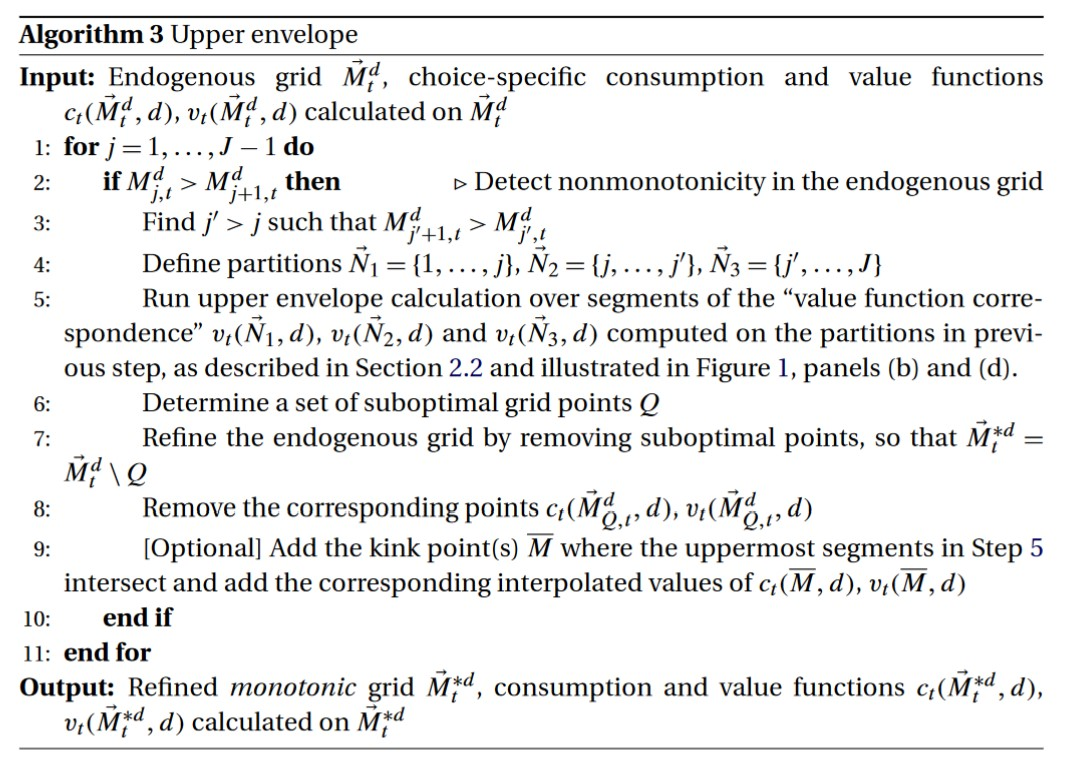
\includegraphics[scale=0.55]{algorithm3.jpg}
	\end{figure}
	\hyperlink{fig:upperenvelope}{\beamerreturnbutton{Figure: Upper Envelope}}
\end{frame}


\end{document}

